\documentclass[dissertation.tex]{subfiles}
\begin{document}

\chapter{Background}

This chapter provides background information on two topics heavily utilized
throughout this dissertation: Western music theory and recurrent neural
networks. It introduce the definitions and notation used in later sections.

\section{A primer on Western music theory}

Music theory is a branch of musicology concerned with the study of the rules
and practices of music. While the general field includes study of acoustic
qualities such as dynamics and timbre, we restrict the scope of our research
and discussion to modeling notes within the musical composition and neglect
issues related to articulation instructions (e.g. staccato, trill, accents) as
well as synthesis/generation of the physical acoustic waveforms.

This is justified because the phsyical waveforms are more closely related
to the skill of the performers and instruments used and are likely to vary
significantly across different performances. Furthermore, articulations in
the same musical piece may differ across transcriptions and performers.
Despite these variations, a piece of music is still recognizable from just the
notes, suggesting that notes are the defining element for a piece of music.

\subsection{Notes: the basic building blocks}

A \emph{note} is the most fundamental element of music composition and
represents a sound played at a certain \emph{pitch} for a certain
\emph{duration}. As a music \emph{score} can be viewed as a collection of notes
along with when they are played (i.e. their \emph{offsets}), notes are the
fundamental building blocks for musical compositions.

\subsubsection{Pitch}

Though pitch is closely related to physical frequency of vibration of a
waveform (as measured in Hertz), pitch its a perceptual property whose semantic
meaning is derived from a listener's perception. This distinction has been
scrutinized by Terhardt
\cite{:/content/asa/journal/jasa/55/5/10.1121/1.1914648}, whose visual analogy
in \autoref{fig:pitch} illustrates how a pitch can be heard even if its
percieved frequency is absent just as one may see the word ``PITCH'' despite
being presented with only a suggestive shadow.

\begin{figure}[htpb]
    \centering
    
\includegraphics[width=0.6\linewidth]{Figures/pitch.pdf}
    \caption{Terhardt's visual analogy for pitch. Similar to how
        the viewer of this figure may percieve contours not present, pitch
        describes subjective information received by the listener even when
    physical frequencies are absent.}
    \label{fig:pitch}
\end{figure}

Despite its psychoacoustic nature, it is nevertheless useful to objectively
quantify pitch as a frequency. To do so, we first need some definitions. The
difference between two frequencies is called an \emph{interval} and an
\emph{octave} is an interval corresponding to the distance between a frequency
$f \in \RR^+$ and its doubling $2f$ or halving $f/2$. Two frequencies spaced
exactly an octave apart are perceived to be similar, suggesting that music is
percieved on a logarithmic scale.

Most Western music is based on the \emph{twelve-note chromatic scale}, which
divides an \emph{octave} into twelve distinct frequencies. The \emph{tuning
system} employed dictates the precise intervals between subdivisions, with
\emph{equal temperament tuning} (all subdivisions are equally spaced on a
logarithmic scale) presently the most widely used
method\cite{denton1997history}. \todo{Talk about well-tempered tuning and bach}
Under twelve-note equal temperament tuning, the distance between two
consecutive subdivisions ($1/12$ of an octave) is called a \emph{semitone}
(British) or \emph{half-step} (North American) and two semitones constitutes
a \emph{tone} or \emph{whole-step}.

When discussing music, \emph{note names} which enable succinct specification of
a musical pitch are often employed. In \emph{scientific pitch notation},
\emph{pitch classes} which represent a pitch modulo the octave are specified by
a letter ($C, D, E, F, G, A, B$) and optionally a single \emph{accidental}. Pitch
classes without accidentals are called \emph{natural} and correspond to the white
keys on a piano. Two accidentals are possible: sharps ($\#$) raise the natural
pitch class up one semitone and flats ($\flat$) lower by one semitone.
\autoref{fig:piano-keys} illustrates how these pitch classes map to keys on a
piano.

\begin{figure}[htpb]
    \centering
    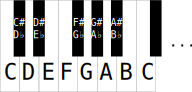
\includegraphics[width=0.6\linewidth]{Figures/piano-keys.pdf}
    \caption{Illustration of an octave in the 12-note chromatic scale
        on a piano keyboard.}
    \label{fig:piano-keys}
\end{figure}

Since pitch classes represent equivalence class of frequencies spaced an
integral number of octaves apart, unambiguously specifying a pitch requires not
only a pitch class but also an octave. In scientific pitch notation, this is
accomplished by appending an octave number to a pitch class letter (see
\autoref{fig:pitch-class}). Together, a pitch class and octave number uniquely
specify the notation for a pitch. On sheet music, the pitch of a note is
indicated by its vertical position with respect to the \emph{stave} (the five
horizontal lines and four spaces).

\begin{figure}[htpb]
    \centering
    \includegraphics[width=0.6\linewidth]{Figures/Pitch_notation.png}
    \caption{Scientific pitch notation and sheet music notation of $C$ notes at
    ten different octaves.  \todo{Cite wiki scientific pitch notation}}
    \label{fig:pitch-class}
\end{figure}

\subsubsection{Transposition invariance}

Note that the discussion of pitch thus far has not made any direct connection
between pitch and frequency. Indeed, this lack of dependence on absolute
physical frequency highlights music's \emph{transposition invariance property}:
many semantically relevant features in music are present the relative relations
between pitches rather than absolute frequencies and hence remain invariant
when the entire piece of music is offset by a constant frequency. However, a
fixed reference frequency is oftentimes required for performance and
reproduction purposes. To convert from pitch notation to physical frequencies,
common modern practice is to tune $A4$ to 440 Hz (a practice known as A440).

In addition to pitch, a note also possesses a \emph{duration}. The duration of
a note indicates how long it is to be played and is measured in fractions of a
\emph{whole note} (American) or \emph{semibreve} (British). Perhaps the most
common duration is a \emph{quarter-note} (American) or \emph{crotchet}
(British). Other note durations are also possible and the most common along
with their notation in sheet music are enumerated in
\autoref{fig:note-durations}. The relationship between durations and
physical time intervals is given by the \emph{tempo}, which is usually
denoted near the start of the piece in beats per minute.

\begin{figure}[htpb]
    \centering
    \includegraphics[width=0.6\linewidth]{Figures/note-durations.png}
    \caption{Comparison of various note durations. \todo{Cite wiki Whole note}}
    \label{fig:note-durations}
\end{figure}

Our work focuses in particular on \emph{tonal music}, a genre of music
characterized by the prevalence of one pitch class (the \emph{tonic}) around
which the melody and harmony are built.

A basic concept within tonal music is the \emph{scale}, which defines a subset
of pitch classes that are ``in key'' with respect to the tonic. Two fundamental
scales are the major (with step pattern
whole-whole-half-whole-whole-whole-half) and minor scales
(whole-half-whole-whole-half-whole-whole). The choice of tonic and scale is
collectively referred to as the \emph{key}. Many musical phenomena such as
stability, mood, expectation, and resolution can be attributed to choice of key
and \emph{modulations} (i.e. changes in key during the middle of a piece of
music).

\section{Neural sequence probability modeling}

Our work in later sections make heavy use of neural networks. In this section,
we briefly review the relevant concepts and set up notation.

\subsection{Neurons: the basic computation unit}

Neurons are the basic abstraction which are combined together to form
neural networks. A \emph{neuron} is a parametric model of a function $f : \RR^D \to
\RR$ from its $D$-dimensional input $\x$ to its output $y$. Our neurons will be
defined as
\begin{equation}
    f(\x) \coloneqq \sigma( \langle \vec{w}, \x \rangle)
\end{equation}
which can be viewed as an inner product with \emph{weights} $\vec{w}$ to
produce an \emph{activation} $z \coloneqq \langle \vec{w}, \x \rangle
\in \RR$ which is then squashed to a bounded domain by a non-linear
\textbf{activation function} $\sigma : \RR \to [L, U]$. This is visually
depicted in \autoref{fig:nn-single}, which also makes apparent the
interpretation of weight $w_i$ as the sensitivity of the output $y$ to the
input $x_i$.

\begin{figure}[htpb]
    \centering
    \input{Figures/nn-single.pdf_tex}
    \caption{A single neuron first computes an activation $z$ and then passes it through
    an activation function $\sigma(\cdot)$}
    \label{fig:nn-single}
\end{figure}

\subsection{Feedforward neural networks}

Multiple neurons may share inputs and have their outputs concatenated together
to form a \emph{layer} modelling a multivariate functions $f :
\RR^{D_\text{in}} \to \RR^{D_\text{out}}$. Multiple layers can then
be composed together to form a \emph{feedforwd neural network}.

\begin{figure}[htpb]
    \centering
    \input{Figures/nn-ffw.pdf_tex}
    \caption{Graph depiction of a feedforward neural network with $2$ hidden layers}
    \label{fig:nn-ffw}
\end{figure}

Although a single hidden layer is theoretically sufficient for a universal
function approximator\cite{Cybenko1993}, the number of hidden units to
guarantee reported theoretical bounds are usually unfeasibly large. Instead,
recent work in \emph{deep learning} has shown that deep models which contain
many hidden layers can achieve strong performance across a variety of
tasks\cite{Bengio2011}.

The improved modeling capacity gained by composing multiple layers is due to
the composition of multiple non-linear activation functions.
In fact, it is easy to show that removing activation functions would make
a deep network equivalent to a single matrix transform: let $\W_{l,l+1}$
denote the weights between layers $l$ and $l+1$. The original neural network
computes the function
\begin{equation}
    \sigma\left(
        \W_{L,L-1} \sigma \left(
            \W_{L-1,L-2}\cdots \sigma \left(
                \W_{2,1} \x
            \right) \cdots
        \right)
    \right)
\end{equation}
After removing the activation functions $\sigma$, we are left with
\begin{equation}
    \W_{L,L-1} \W_{L-1,L-2}\cdots \W_{2,1} \x
    = \x
    = \tilde{\W} \x
\end{equation}
where $\tilde{\W} = \left(\prod_{i=1}^{L-1} \W_{i,i+1} \right)$
is a matrix transform computing the same function as the neural network with
activation functions removed.

\subsection{Recurrent neural networks}

While feedforward neural networks provide a flexible model for approximating
arbitrary functions, they require a fixed-dimension input $\x$ and hence
cannot be directly applied to sequential data $\x = (\x_t)_{t=1}^T$ where $T$ may
vary.

A naive method for extending feedforward networks would be to independently
apply a feedforward network to compute $\y_t = f(\x_t \theta)$ at each timestep
$1 \leq t \leq T$. However, this approach is only correct when each output
$\y_t$ depends only on the input at the current time $\x_t$ and is independent of
all prior inputs $\{\x_k\}_{k < t}$. This assumption is false in musical data:
the current musical note usually is highly dependent on the sequence of notes
leading up to it.

This shortcoming motivates \emph{recurrent neural networks} (RNNs), which
generalize feedforward networks by introducing time-delayed recurrent
connections between hidden layers (Elman networks \cite{elman1990finding}) or
from the output layers to the hidden layers (Jordan networks
\cite{jordan1997serial}). \autoref{fig:nn-rnn} illustrates an Elman-type
network. Notice that apart from the edges between hidden nodes, the network is
identical to a regular feedforward network (\autoref{fig:nn-ffw}).

\todo{Why do we use Elman}

\begin{figure}[htpb]
    \centering
    \input{Figures/nn-rnn.pdf_tex}
    \caption{Graph representation of an Elman-type RNN.}
    \label{fig:nn-rnn}
\end{figure}

To apply the RNN over an input sequence $\x$, the activations of the hidden
states are first initialized to an initial value $\h \in \RR^{D_{h}}$. Next,
for each timestep $t$ the hidden layer activations are computed using the
current input $\x_t$ and the previous hidden state activations $\h_{t-1}$.
This motivates an alternative perspective on RNNs as a template consisting
of a feedforward network with inputs $\{\x_t, \h_{t-1}\}$ (see
\autoref{fig:rnn-elman}) replicated across time $t$.

\begin{figure}[htpb]
    \centering
    \input{Figures/nn-rnn-elman.pdf_tex}
    \caption{Equivalent formulation of an Elman-type RNN treating the
    time-delayed hidden state $\h_{t-1}$ as additional inputs to a feedforward
    network}
    \label{fig:rnn-elman}
\end{figure}


\subsubsection{Memory cell abstraction}

Notice that \autoref{fig:rnn-elman} delineates the recurrent hidden state from
the rest of the diagram, introducing an abstraction called a \emph{memory
cell}. This allows us to abstract away how $\y_t$ and $\h_t$ are computed from
$\x_t$ and $\h_{t-1}$, enabling discussion of RNNs applicable to many different
implementations. Concretely, A memory cell is an interface which for each
timestep $t$:
\begin{itemize}
    \item Takes inputs
        \begin{itemize}
            \item The current element in the input sequence $\x_t$
            \item The previous hidden state $\h_{t-1}$
        \end{itemize}
    \item Produces outputs
        \begin{itemize}
            \item The next  hidden state $\h_t = f_h (\x_t, \h_{t-1})$
            \item The outputs $\y_t = f_y (\h_t)$.
        \end{itemize}
\end{itemize}
In future diagrams, we will abstractly represent the memory cell
as a node labelled with $\h$.

\subsubsection{Unrolling into a DAG}

One important operation on RNNs is \emph{unrolling} the template in
\autoref{fig:rnn-elman} into a chain of $T$ replications with connected hidden
states (\autoref{fig:rnn-single-unrolled}). This removes the time-delayed
recurrent, converting the RNN into a finite directed acyclic graph where nodes
represent pieces of data and edges $s \to t$ indicate that $t$ is a function of
$s$. This is identical to a feedforward network, justifying the view of RNNs as
a dynamically-sized feedforward network with $T$ layers and parameters tied
across all layers.

\todo{Talk about how view of unrolled RNN as DNN inspires cross-polination e.g.
gating to let information flow deeper: LSTM gates and highway networks, grid
LSTMS}

\begin{figure}[htpb]
    \centering
    \resizebox{4.5in}{!}{\input{Figures/rnn-single-unrolled.pdf_tex}}
    \caption{Signal flow diagram representation of a single-layer RNN and its corresponding
    directed acyclic graph after unrolling}
    \label{fig:rnn-single-unrolled}
\end{figure}

\autoref{fig:rnn-single-unrolled} makes it obvious how the hidden state is
carried along throughout the sequence of computations, giving rise to a useful
alternative interpretation of the hidden state as a temporal memory mechanism.
Under this interpretation, we can view the hidden state update $\h_t = f_h
(\x_t, \h_{t-1})$ as \emph{writing} information extracted from the
current inputs $\x_t$ to the memory $\h_{t-1}$. Similarly, producing
the outputs $\y_t = f_y (\h_t)$ can be seen as \emph{reading}
information from the hidden state.

\todo{Compare to N-grams; show how it's like an infinite context. One
    interpretation is to view the hidden state $\h_t$ as an
    infinite-length prior context window, summarizing all of the prior inputs
    into into a compact fixed-size vector.}

\subsubsection{Stacking memory cells to form multi-layer RNNs}

Since the RNN outputs $\y$ also form a sequence with the same length as
the inputs $\x$, they can be used as inputs into another RNN. This
stacking of multiple memory cells is similar to the layering seen in deep
neural networks, giving rise to the term \emph{deep neural sequence models}
\todo{Cite?}. This is illustrated in \autoref{fig:rnn-multi-unrolled}.

\begin{figure}[htpb]
    \centering
    \resizebox{4.5in}{!}{\input{Figures/rnn-multi-unrolled.pdf_tex}}
    \caption{Template and unrolling of a stacked 2-layer RNN}
    \label{fig:rnn-multi-unrolled}
\end{figure}

The greater modeling capabilities of multilayer RNNs can be attributed to two
primary factors: composition of multiple non-linearities and an increase in the
number of paths through which information can flow. The former is analogous to
the feedforward case: stacking memory cells increases the number of
non-linearities in the composite cell just like stacking multiple layers in
feedforward networks. To understand the latter point, notice that in
\autoref{fig:rnn-single-unrolled} there is only a single path from
$\x_{t-1}$ to $\y_{t}$ hence the conditional independence
$\y_{t} \independent \x_{t-1} | \h^{(1)}_t$ is satisfied.
However, in \autoref{fig:rnn-multi-unrolled} there are multiple paths from
$\x_{t-1}$ to $\y_{t}$ (e.g. passing through either
$\h^{(2)}_{t-1} \to \h^{(2)}_t$ or $\h^{(1)}_{t-1} \to
\h^{(1)}_t$) through which information may flow. Additionaly, the
hidden state transitions occur on two seperate memory cells so parameters
need not be tied and the stacked RNN can learn different time dynamics
at each depth.

\subsection{Training RNNs: backpropogation through time}

Mathematically, a RNN is a discrete time dynamical system commonly
parameterized as:
\begin{eqnarray}
    \h_t &=& \W_{xh} \sigma_{xh} \left( \x_t \right) + \W_{hh} \sigma_{hh} \left( \h_{t-1} \right) \label{eq:rnn-ht}\\
    \y_t &=& \W_{hy} \sigma_{hy} \left( \h_t \right) \label{eq:rnn-yt}
\end{eqnarray}
where $\sigma_{\cdot \cdot}(\cdot)$ are activation functions acting element-wise
and the parameters $\theta = \{ \W_{xh}, \W_{hh}, \W_{hy}\}$
are learned from data to minimize a cost $\mathcal{E} = \sum_{1 \leq t \leq T}
\mathcal{E}_t(\x_t)$ measuring the performance of the network on some task.

One approach for computing the necessary gradients is \emph{backpropogation through
time} (BPTT)\cite{At}, an adaptation of the backpropogation algorithm \todo{cite}
to the unrolled RNN computation graph. Letting $\theta$ denote the model parameters,
we can apply the chain rule to the unrolled RNN's computation graph
in \autoref{fig:rnn-bptt} to obtain
\begin{eqnarray}
    \frac{\pd \mathcal{E}}{\pd \theta} &=& \sum_{1 \leq t \leq T} \frac{\pd \mathcal{E}_t}{\pd \theta} \\
    \frac{\pd \mathcal{E}_t}{\pd \theta} &=& \sum_{1 \leq k \leq t} \left(
        \frac{\pd \mathcal{E}_t}{\pd \y_t}
        \frac{\pd \y_t}{\pd \h_t}
        \frac{\pd \h_t}{\pd \h_k}
        \frac{\pd \h_k}{\pd \theta}
    \right) \label{eq:error-t}\\
    \frac{\pd \h_t}{\pd \h_k} &=&
    \prod_{t \geq i > k} \frac{\pd \h_i}{\pd \h_{i-1}}
    = \prod_{t \geq i > k} \W_{hh}^\tp \diag \left( \sigma_{hh}'( \h_{i-1} ) \right)
    \label{eq:error-transfer}
\end{eqnarray}

\begin{figure}[htpb]
    \centering
    \input{Figures/rnn-bptt.pdf_tex}
    \caption{The gradients passed along network edges during BPTT.}
    \label{fig:rnn-bptt}
\end{figure}

\autoref{eq:error-t} expresses how the error $\mathcal{E}_t$ at time $t$ is a sum
of \emph{temporal contributions} $
\frac{\pd \mathcal{E}_t}{\pd \y_t}
\frac{\pd \y_t}{\pd \h_t}
\frac{\pd \h_t}{\pd \h_k}
\frac{\pd \h_k}{\pd \theta}$
measuring how $\theta$'s impact on $\h_k$ affects the cost at some future
time $t > k$. The factors in \autoref{eq:error-transfer} measures the affect
of the hidden state $\h_k$ on some future state $\h_t$ where $t > k$
and can be interpreted as transferring the error ``in time'' from step $t$ back
to step $k$ \cite{Pascanu2012}.

\subsubsection{Vanishing/exploding gradients}

Unfortunately, naive implementations of \autoref{eq:rnn-ht} and
\autoref{eq:rnn-yt} oftentimes suffers from two well known problems: the
\emph{vanishing gradient} and \emph{exploding gradient}\cite{Bengio1994}.
Broadly speaking, these problems are both related to the product in
\autoref{eq:error-transfer} exponentially growing or shrinking for long
timespans (i.e. $t \gg k$).

Following Pascanu \textit{et al.} \cite{Pascanu2012}, let $\| \cdot \|$ be any
submultiplicative matrix norm (e.g. Frobenius, spectral, nuclear, Shatten
$p$-norms). Without loss of generality, we will use the \emph{operator norm}
defined as
\begin{equation}
    \| A \| = \sup_{x \in \RR^n; x \neq 0} \frac{|A x|}{|x|}
\end{equation}
where $|\cdot|$ is the standard Euclidian norm.

From submultiplicativity, we have that for any $k$
\begin{equation}
    \left\| \frac{\pd \h_k}{\pd \h_{k-1}} \right\|
    \leq \| \W_{hh}^\tp \| \| \diag\left( \sigma_{hh}'(\h_{k-1}) \right) \|
    \leq \gamma_{\W} \gamma_\sigma
\end{equation}
where we have defined $\gamma_{\W} = \| \W_{hh}^\tp \|$ and
\begin{align}
    \gamma_\sigma
    &\coloneqq \sup_{h \in \RR^n} \| \diag \left( \sigma_{hh}'(\h) \right) \|  &\\
    &= \sup_{h \in \RR^n} \max_i \sigma_{hh}'(\h)_i &\mbox{Operator norm of diag} \\
    &= \sup_{x \in \RR} \sigma_{hh}'(x) &\mbox{$\sigma_{hh}$ acts elementwise}
\end{align}

Substituting back into \autoref{eq:error-transfer}, we find that
\begin{equation}
    \left\| \frac{\pd \h_t}{\pd \h_k} \right\|
    = \left\| \prod_{t \geq i > k} \frac{\pd \h_i}{\pd \h_{i-1}} \right\|
    \leq  \prod_{t \geq i > k} \left\| \frac{\pd \h_i}{\pd \h_{i-1}} \right\|
    \leq (\gamma_{\W} \gamma_\sigma)^{t-k}
\end{equation}

Hence, we see that a sufficient condition for vanishing gradients is
for $\gamma_{\W} \gamma_\sigma < 1$, in which case $\left\| \frac{\pd \h_t}{\pd \h_k} \right\| \to 0$
exponentially for long timespans $t \gg k$. $\qed$

For common activation functions, $\gamma_\sigma$ is bounded and reasonably
small (e.g. $\gamma_\sigma = 1$ for $\sigma_{hh} = \tanh$, $\gamma_\sigma =
0.25$ for $\sigma_{hh} = \sigmoid$). This enables us to write the sufficient
condition for vanishing gradients as
\begin{equation}
    \gamma_{\W} = \| \W_{hh}^\tp \| \leq \frac{1}{\gamma_\sigma}
    \label{eq:vanishing-gradients-suff}
\end{equation}
The converse of the proof implies that $\| \W_{hh}^\tp \| \geq
\frac{1}{\gamma_\sigma}$ are necessary conditions for $\gamma_{\W}
\gamma_\sigma > 1$ and exploding gradients to occur.

\subsection{Long short term memory: solving the vanishing gradient}

As \autoref{eq:vanishing-gradients-suff} provide sufficient conditions for
vanishing gradients, any model which we may hope to successfuly learn long range
dependencies must have $\gamma_{\W} \gamma_\sigma \geq 1$.

The \emph{long short term memory} (LSTM) model was proposed by Hochreiter and
Schmidhuber \cite{hochreiter1997long} as a method for dealing with
the vanishing gradient problem. It does so by enforcing \emph{constant error flow}
on \autoref{eq:error-transfer}, that is
\begin{equation}
    \W_{hh}^\tp \sigma_{hh}' (\h_{t}) = \matr{I}
\end{equation}
where $\matr{I}$ is the identity matrix.

Integrating the above differential equation yields $\W_{hh} \sigma_{hh}(\h_{t}) = \h_{t}$.
Since this should hold for any hidden state $\h_{t}$, this means that:
\begin{enumerate}
    \item $\W_{hh}$ must be full rank
    \item $\sigma_{hh}$ must be linear
    \item $\W_{hh} \circ \sigma_{hh} = \matr{I}$
\end{enumerate}
In LSTMs, this is ensured by setting $\sigma_{hh} = \W_{hh} = \matr{I}$, effectively removing
time dynamics from the hidden state. In the literature, this is referred to as
the \emph{constant error carousel} (CEC).

In addition to the CEC, LSTMs possess three sets of gates controlling access to
the CEC:
\begin{itemize}
    \item \textbf{Input gate}: scales input $x_t$ elementwise by $i_t \in [0,1]$, \emph{writes} to $h_t$
    \item \textbf{Output gate}: scales output $y_t$ elementwise by $o_t \in [0,1]$, \emph{reads} from $h_t$
    \item \textbf{Forget gate}: scales previous cell value $h_{t-1}$ by $f_t \in [0,1]$, \emph{resets} $h_t$
\end{itemize}
These gates imbue the model with the ability to read, write, and reset the hidden state.
This mirrors the instructions available on memory abstractions in models of computation,
motivating the view that a LSTM is learning a ``program'' which computes $\y$
from $\x$ \cite{hochreiter1997long}.

Mathematically, LSTM is defined by the following set of equations:
\begin{eqnarray}
    \i_t &=& \sigmoid(\W_{xi} \x_t + \W_{yi} \y_{t-1} + \b_i) \\
    \o_t &=& \sigmoid(\W_{xo} \x_t + \W_{yo} \y_{t-1} + \b_o) \\
    \f_t &=& \sigmoid(\W_{xf} \x_t + \W_{yf} \y_{t-1} + \b_f) \\
    \h_t &=& \f_t \odot \h_{t-1} + \i_t \odot \tanh(\W_{xh}\x_t + y_{t-1} \W_{yh} + \b_h) \label{eq:lstm-dynamics} \\
    \y_t &=& \o_t \odot \tanh(\h_t)
\end{eqnarray}
where $\odot$ denotes elementwise multiplication of vectors.
\autoref{fig:lstm-cell} depicts a single LSTM cell. Notice that it implements
the memory cell interface, so the prior discussion on RNNs is applicable here.

\begin{figure}[htpb]
    \centering
    \input{Figures/lstm-unit-2.pdf_tex}
    \caption{Schematic for a single LSTM cell.}
    \label{fig:lstm-cell}
\end{figure}

Some authors define LSTMs such that $\h_t$ is not used to compute gate
activations, referring to the case where $\h_t$ is connected as ``peephole
connections''\cite{gers2002learning}. We will use \emph{LSTM} to refer to the
system of equations given above.

As a consequence of \autoref{eq:lstm-dynamics}, 
LSTMs protect from vanishing gradient, but not exploding gradient. Research has shown
that gradient clipping is essential to permit successful applications \cite{Pascanu2012}.
\begin{enumerate}
    \item
\end{enumerate}

\todo{Truncated BPTT}
\todo{Gradient clipping for avoiding exploding gradient}

\printbibliography

\end{document}
